\documentclass[tikz]{standalone}
\usepackage{tikz}
\usetikzlibrary{positioning, graphs}
\usetikzlibrary{graphs.standard}
\begin{document}
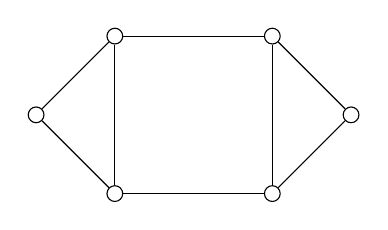
\begin{tikzpicture}
		[every node/.style={draw,circle,inner sep = 0mm, minimum size = 2mm}]
		\node at (0,0) (a) {};
		\node at (1,1) (b) {};
		\node at (1,-1) (c) {};
		\node at (3,1) (d) {};
		\node at (3,-1) (e) {};
		\node at (4,0) (f) {};
		
		\draw (a) -- (b);
		\draw (a) -- (c);
		\draw (b) -- (d);
		\draw (b) -- (c);
		\draw (c) -- (e);
		\draw (e) -- (d);
		\draw (e) -- (f);
		\draw (d) -- (f);
\end{tikzpicture}
\end{document}